\documentclass{report}

\usepackage[utf8]{inputenc}
\usepackage[T1]{fontenc}
\usepackage[francais]{babel}
\usepackage{graphicx}
\usepackage{hyperref}
\usepackage{textcomp}
\usepackage{amsmath}
\usepackage{geometry}
\usepackage{pdfpages}

\usepackage{matlab-prettifier}

\usepackage{array,multirow,makecell}
\setcounter{secnumdepth}{3}
\setcounter{tocdepth}{3}
\setcellgapes{4pt}
\makegapedcells
\newcolumntype{R}[1]{>{\raggedleft\arraybackslash }b{#1}}
\newcolumntype{L}[1]{>{\raggedright\arraybackslash }b{#1}}
\newcolumntype{C}[1]{>{\centering\arraybackslash }b{#1}}

\usepackage[pages=some]{background}
\backgroundsetup{
	scale=1,
	color=black,
	opacity=0.1,
	angle=0,
	contents={%
		
\includegraphics[width=\paperwidth,height=\paperheight]{img/ulbback.jpg}
	}%
}


\title{\Huge\emph{Cooling Down a Coke Can}\\
	\LARGE Experiment study\\
	\vspace{11pt}
	\large Fluid Mechanics and Transport Processes}

\date{December 2015}

\author{Nathan DE PRYCK \and Miquel KEGELEIRS \and Mischa MASSON}



\begin{document}
	
	\begin{figure}[t]
		
\includegraphics[width=15cm]{img/entete.PNG}
	\end{figure}
	
	\maketitle
	
	\renewcommand{\abstractname}{``Cooling down a coke can'' \\Experiment study by Nathan De Pryck, Miquel Kegeleirs and Mischa Masson\\ Université Libre de Bruxelles\\2015-2016.}
	
	\BgThispage
	
	\begin{abstract}
		TO BE WRITTEN
	\end{abstract}
	
	\clearpage
	
	\tableofcontents
	
	\chapter{Introduction}\label{intro}
	
	This report tends to explain the experiment done the 06/10/2015 during the "Fluid Mechanics and Transport Processes" course at ULB.The experiment can be found at \hyperref{https://www.youtube.com/watch?v=MSwc_IAPh3E}{}{}{this address}\footnote{\url{https://www.youtube.com/watch?v=MSwc_IAPh3E}}.
	The physical phenomena behind this experiment are related to the heat transfert processes.

	The experiment consists to take three coke cans and a bucket of ice and water.
	Each can is submited to a different treatment. The first can is used to determine the initial temperature. The second is just put inside
	the bucket mentionned before and the last coke can is spun inside the bucket with a speed of $1000rpm$. The duration of the experiment is $60$ seconds.
	At the end of this duration, the temperature of each coke can is measured. 
	
	The result for the 06/10/2015 experiment were : 16 \textdegree C for the first can, 11.9 \textdegree C for the second and 11 \textdegree C for the spinning can. 
	The question here is how to explain this difference of temperature and the answer can be given by two phenomena : conduction and convection.

	Both of those phenomena will be explained in the first part of this report. The second pard will describe the different mathematical models used for both cases. 
	The simplifying assumptions considered for the global experiment will also be justified. 
	The third part will tend to explain the reasons of the differences between the numerical data obtained and the measurements taken during the manipulation. 
	A global conclusion will finish these report.
	
	\begin{itemize}
		\item Three coke cans were available as well as a bucket of ice and water (at 0\textcelsius) and a drill to spin the can inside the bucket.
		\item One of the cans was used to determine the initial temperature (16\textcelsius) of the fluid (essentially water) inside the can.
		\item One can was left inside the bucket for 60 seconds and a final temperature of 11.9\textcelsius \ was measured as a result of the conductive heat transfer with the surrounding fluid.
		\item One can was spun inside the bucket for 60 seconds at about 1000 rounds per minute, and a final temperature of 11\textcelsius \ was measured as a result of the convective and conductive heat transfer.
	\end{itemize}
	
	In the first chapter, convective and conductive processes that are related to the experiment will be described. Those phenomena will then be applied to the problem via a mathematical model, including a discussion of simplifications brought to the problem in order to simplify calculations. This model will be compared to the experimental results, then a discussion on it's reliability followed by a conclusion on mathematical models in general will be presented.
	
	\chapter{Heat transfer processes}\label{htp}
	
	They are three different ways of transferring heat: conduction, convection and radiation. Due to its nature (heat exchange between two distant bodies at very different temperatures), radiation can be neglected for this experiment and will thus not be presented here.
	
	\section{Conduction}\label{cd}
	
	Thermal conduction is a heat transfer process without macroscopic movement of matter. It is initiated by a difference of temperature between contiguous bodies (or inside a body). This difference of temperature implies a difference of internal energy : the energy is higher in the warmer area than in the cooler. By diffusion and collisions between the particles, which can be molecules in a fluid or conduction electrons in a solid, particles in the warmer area transfer kinetic energy to the other particles, and make them move and/or vibrate faster. This creates a heat flow from the warmer area to the cooler until the system reaches thermal equilibrium. Furthermore, conduction is an irreversible process.
	
	Conduction is described by the following general equation, which is demonstrated in Professor Jean-Marie Buchlin's course\cite{Buchlin}, Chapter 13.
	
	\begin{equation}
		\frac{\delta T}{\delta t} = \bigtriangledown . (\alpha \bigtriangledown T)+ \dot{Q}_v
	\end{equation}
	
	This equation can not be used by itself because of it's nature (second degree partial derivative equation). It thus needs boundary conditions linked to properties of the system. Those can be geometrical, physical, temporal or border conditions.
	
	Boundary conditions used and simplifications of the above presented general equation will be discussed in chapter~\ref{mm}.
		
	\section{Convection}\label{cv}
	
	Convection refers to particular heat transfers in fluids. Convection occurs when some fluid is in movement. The movement lead to an advection (heat is transported by moving matter).
	
	Convection is described as following :
	\begin{equation}
		Convection = Conduction + Advection
	\end{equation}
	
	Therefore, it is easy to understand that convection is superior than conduction in fluids in a flux situation. 
	
	An important distinction can be made in convective heat transfers : convection can be natural or forced.
	Natural convection occurs mainly due to temperature differences which modify fluids density. Increasing the temperature amplifies thermal agitation which leads to a volume expansion along with a decreasing of density. Cold components are thus heavier and fall down while lighter hot components rise. This created a bulk fluid motion initiating a convective heat transfer called natural convection.
	Forced convection refers to a convective heat transfer due to surface forces which generates a movement in the fuid. This convective heat transfer has thus a great sensitivity to the velocity acquired by the fluid. The surfaces forces can be applied by either artificial ways such as fans or natural ways such as blowing wind. 
	Both natural and forced convection can happend simultaneously but forced convection is usually the most significant, especially at high velocity.
	
	The flow properties also have a major impact on convective heat transfers and can be expressed through dimensionless numbers.
	As convection depends on the flow (laminar, turbulent,...), we will discuss the equation to use in the next chapter.
	
	\chapter{Mathematical model}\label{mm}
	
	The idea behind mathematical models is to create a simplified version of a problem, that is accurate enough to predict the behaviour of a system, and at the same time simple enough to be resolved with few calculations.
	
	This means that some simplifications of the above mentioned equations can be made, using the properties of the studied system.
	
	General simplifying assumptions for the experiment will first be described and their validity will be discussed, then two simplified models will be presented: one for the non-spinning can and one for the spinning can.
	
	\section{General simplifying assumptions}\label{gsa}
	
	The first assumption that will be considered is that the fluid contained in the can has properties similar to those of water. Coke is indeed an aqueous solution containing sugar and other ingredients, but at relatively low concentrations.
	Properties of water can be found in annex~\ref{WTPP} and are extracted from \emph{``Perry’s Chemical Engineers’ Handbook''\cite{properties}}.
	
	We also assume that the can is a perfect cylinder with an height of $h=116mm$ and a diameter of $d=66mm$\footnote{Those dimensions are standard for European Aluminium $330ml$ cans and can be found on \hyperref{http://www.webpackaging.com/en/portals/rexam/assets/11059498/spec-alu-202/}{}{}{webpackaging.com}}. In reality, the shape of a can is a bit different in order to support pressure but this difference should not be significant in our calculations. The material used for cans is Aluminium and since it is extremely thin(less than $1mm$) and has an excellent thermal conductivity ($>200\frac{W}{K.m}$), its influence on heat transfers can be neglected. The considered model will thus be a cylinder of water laid under water maintained at another temperature and without any exchange of matter, as shown in figure~\ref{cyl}.
	
	\begin{figure}
		\centering
		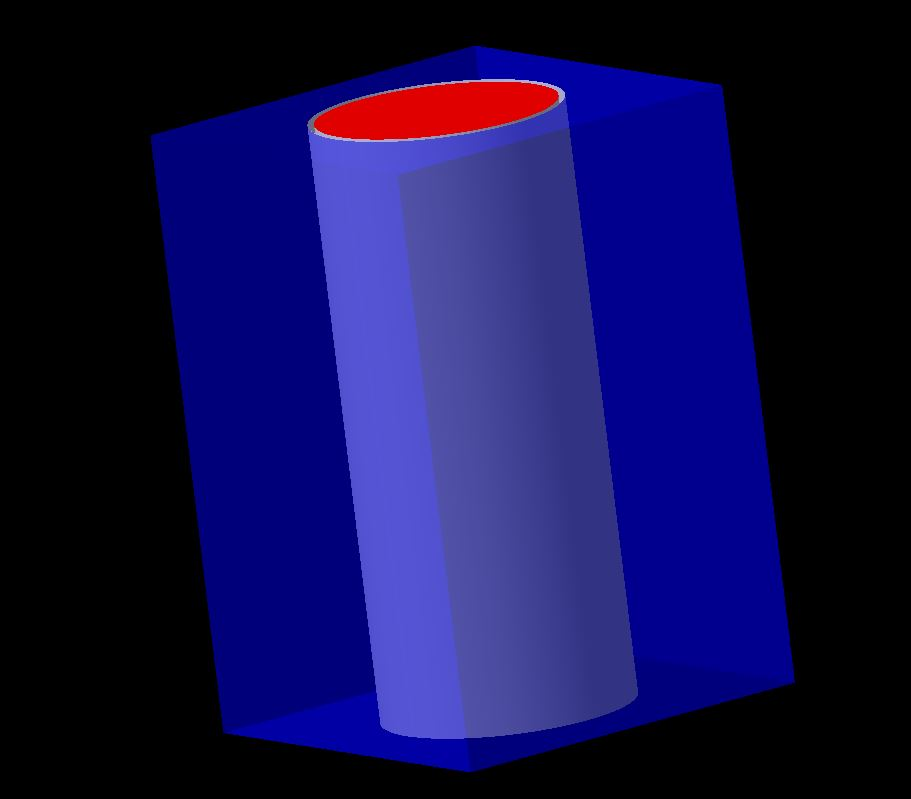
\includegraphics[width=.5\textwidth]{img/cyl.jpg}
		\caption{The red cylinder is hotter water, the blue box is colder water. No matter exchanges, only heat transfer.}
		\label{cyl}
	\end{figure}
	
	Furthermore, the hypothesis that all heat exchanges between the can and the surrounding ice-cold water take place on de sides of the can and not on it's top or bottom will be assumed. The total surface of the can is given by:
	
	\begin{equation}
	\begin{gathered}
		Surface= 2.Surface_{circle} + Surface_{rectangular side} \\
		\Leftrightarrow S= 2 (\pi  (\frac{d}{2})^2) + \pi dh \\
		\Leftrightarrow S= 30.8944 cm^3
	\end{gathered}
	\end{equation}
	
	Bottom and top circular surfaces have a total surface of $2xSurface_{circle}=2 (\pi  (\frac{d}{2})^2)= 6.8424 cm^3$, which makes around $22.14\% $ of the total surface. The reason why it was decided to ignore such a large portion of the can's area is that half of it is not even in contact with ice during the experiment (the system holding the can covers it's top and the non-spinning can is not totally in ice), reducing the area to consider at about $11\% $ of total exchange area. This can still be seen as a large percentage. However, on one side we are trying to cool down a liquid on the bottom of the can and, on the other hand, cold fluids tend to be more dense than hot fluids. Therefore, the liquid in contact with the bottom part will be cooler, making the heat transfer far less efficient there.
	
	The last general simplification made for this experiment is to consider the mix of ice and water surrounding the can as a continuous layer of water maintained at 0\textcelsius. This should be correct enough considering that there is a large quantity of melting ice in an isolated box. Indeed, liquid water is more flexible than ice, the can has a larger surface in contact with molten ice (thus water) than with the ice itself.
	
	
	\section{Simplified models}\label{sm}
	
	With these four simplifications in mind, two models will now be build, one for the non-spinning can and one for the spinning can.
	
	\subsection{Non-spinning can}\label{nsc}
	
	Heat transfer processes in presence are conduction and natural convection. Natural convection appears because of the density change of fluid related to temperature: the cooler the fluid, the denser it is. There is no forced convection because there is no flux in the fluid.
	
	The convective heat transfer coefficient for natural convection (in the can) is given by:
	\begin{equation}
		h_x=Ra^\alpha = cGr^\alpha Pr^\alpha
	\end{equation}
	
	Where $Gr$ is the Grashof number and $Pr$ the Prandtl number. Prandtl can be found in annex~\ref{WTPP}: water being at 16\textcelsius (about $290K$), it gives $Pr=7.56$.\\
	Grashof number is calculated using the following formula (taken from annex~\ref{FORMU}):
	\begin{equation}
	Gr=\frac{\beta g \Delta T_{ref} d^3}{\nu^2}
	\end{equation}
	
	Where:
	\begin{itemize}
		\item $\beta$ is the volume expansion coefficient, given by $\frac{1}{\rho}\frac{\delta\rho}{\delta T}$. Using the tables in annex~\ref{WTPP}, the following approximation can be made : $\beta=1.001\times 10^{-3}\frac{\frac{1}{1.000\times 10^{-3}}-\frac{1}{1.001\times 10^{-3}}}{5}=1.998\times 10^{-4} K^{-1}$.
		\item $g=9.81\frac{m^2}{s}$ is gravity.
		\item $\Delta T_{ref}=16-0=16$\textcelsius\ is the difference of temperature between the water inside the can and the ice-cold water outside of it.
		\item $d=66\times 10^{-3}m$ is the diameter of the cylinder.
		\item $\nu=\frac{\mu}{\rho}=\frac{1080\times 10^{-6}}{\frac{1}{1.001\times 10^{-3}}}=1.081\times 10^{-6}\frac{m^2}{s}$ is water's kinematic viscosity.
	\end{itemize}
	All values used in our calculation can be verified in annex~\ref{WTPP}.
	
	
	Rayleigh number is thus: 
	\begin{equation}
		Ra = GrPr= 7.56\times \frac{1.998\times 10^{-4}\times 9.81\times 16\times (66\times 10^{-3})^3}{(1.081\times 10^{-6})^2}= 5.8329\times 10^{7}
	\end{equation}
	Since $Ra<10^9$, the laminar case can be considered. Assuming that the ice-cold water around the can is at a constant temperature, it is now needed to determine which equation to use for Nusselt number.
	
	The easiest approximation is to describe the cylinder as a rectangular enclosure, with H (the height of the enclosure) equal to $h=116mm$ and L (the characteristic length of the enclosure) equal to $\frac{d}{2}=33mm$. This gives an H on L ratio of $\frac{H}{L}=3.352$. The equation 9-53 at page 555 of ``Heat and Mass Transfer: Fundamentals and Applications''~\cite{HaMT}, chapter 9-5 will thus be used:
	\begin{equation}
		\begin{gathered}
		Nu=0.22(\frac{Pr}{0.2+Pr}Ra)^{0.28}(\frac{H}{L})^{-1/4}\\
		\Leftrightarrow Nu=2.3835\times 10^{1}
		\end{gathered}	
	\end{equation}
	and:
	\begin{equation}
		\begin{gathered}
		Nu=\frac{hL}{k}\\
		\Leftrightarrow h=\frac{Nu k}{L}=\frac{2Nu k}{d}\\
		\Leftrightarrow h=4.3191\times 10^2 \frac{W}{m^2K}
		\end{gathered}	
	\end{equation}
	
	Biot number is given by $Bi=\frac{hL}{k}=\frac{hd}{2k}=23.8347 > 1$. This indicates that \emph{the system can not be considered as a Lumped system}, the temperature inside the can is not homogeneous. But, as the temperature is measured manually by putting a thermometer inside the can, and as the size of the thermometer is not negligible compared to the small radius of the can, the system will be simplified by using the equations for a Lumped system in the case of sensible heat transfer:
	
	\begin{equation}\label{lumped}
		\begin{gathered}
		\rho C_pV\frac{dT}{dt}=-hS_{tot}(T-T_{ext})\\
		\Leftrightarrow \frac{hS_{tot}}{\rho C_pV}dt=\frac{1}{(T_{ext}-T)}dT\\
		\Leftrightarrow \frac{4h}{\rho C_pd}dt=\frac{1}{(T_{ext}-T)}dT\\
		\Leftrightarrow \frac{4h}{\rho C_pd}t=ln(\frac{T_0-T_{ext}}{T_f-T_{ext}})\\
		\Leftrightarrow e^{\frac{4h}{\rho C_pd}t}=\frac{T_0-T_{ext}}{T_f-T_{ext}}\\
		\Leftrightarrow T_f=T_{ext}+\frac{T_0-T_{ext}}{e^{\frac{4h}{\rho C_pd}t}}
		\end{gathered}
	\end{equation}
	
	Using the parameters of the experiment, this gives $T_f=284.14K=10.99$\textcelsius\ after $t=60s$.
	
	The fact that this value is quite far from what is observed in the experiment is due to some simplifications made here, like, for example, using the Lumped system equations, or some of the parameters choice.
	
	Looking at the parameters, the approximation made for $\beta$ can be refined if, instead of using the value approximated over the temperature interval, the value for $\beta$ at 15\textcelsius\ given in Appendix A-1, table A-9 of ``Heat and Mass Transfer: Fundamentals and Applications''~\cite{HaMT}: $\beta=1.38\times 10^{-4} K^{-1}$, is used. Injecting this in the model already adds some accuracy, with a temperature of $11.40$\textcelsius\ ($284.55K$).
	
	Moreover, the values of $\beta$ and $Pr$ are not fixed, they depend on temperature. To get even more accurate results, ``mean values'' of those two numbers will be taken. In order to do so, since their evolution is small in the interval of temperatures ($1.38\times 10^{-4}$ to $0.733\times 10^{-4}$ for $\beta$ and $8.09$ to $9.45\times 10^{-4}$ for Prandtl~\footnote{Be warned that the values for Prandtl are different than the one used before: this is due to the fact that it was decided to use values from the same source (``Heat and Mass Transfer: Fundamentals and Applications''~\cite{HaMT}) here to ensure they are calculated the same way. This also shows the differences that can be observed for the same number, depending of the source and the temperatures it uses as standards}), the assumption is made that their variation is linear and that the linear mean value on the interval can be used. In the end, it gives $\beta=1.056\times 10^{-4} K^{-1}$ and $Pr=8.77$.
	
	The same correction is used for $k$, $\rho$ and $C_p$; values for those parameters become $k=0.584\frac{W}{mK}$, $\rho=999.4\frac{kg}{m^3}$ and $C_p=4189.5\frac{J}{kgK}$.
	
	Those corrections, when injected in the model, give $T_f=284.77K=11.62$\textcelsius\ after $t=60s$. Biot number for this case is $Bi=20.8$, still high. Even with this high Biot number, the value obtained seems acceptable, considering the simplifications made on the system. The error compared to the experimental result is about $2.38$\textdiscount (when taken in degrees Celsius), and the fact that the temperature measurement made during the experiment where not immediate and that the thermometer itself was warm has to be taken in account.
	
	The code used for this part of the model can be found in annex~\ref{codeNS}
	
	
	Graph~\ref{NSg} gives the evolution of temperature($K$) with time($s$) for the last model with enhanced approximations of water's parameters.
	\begin{figure}
		\centering
		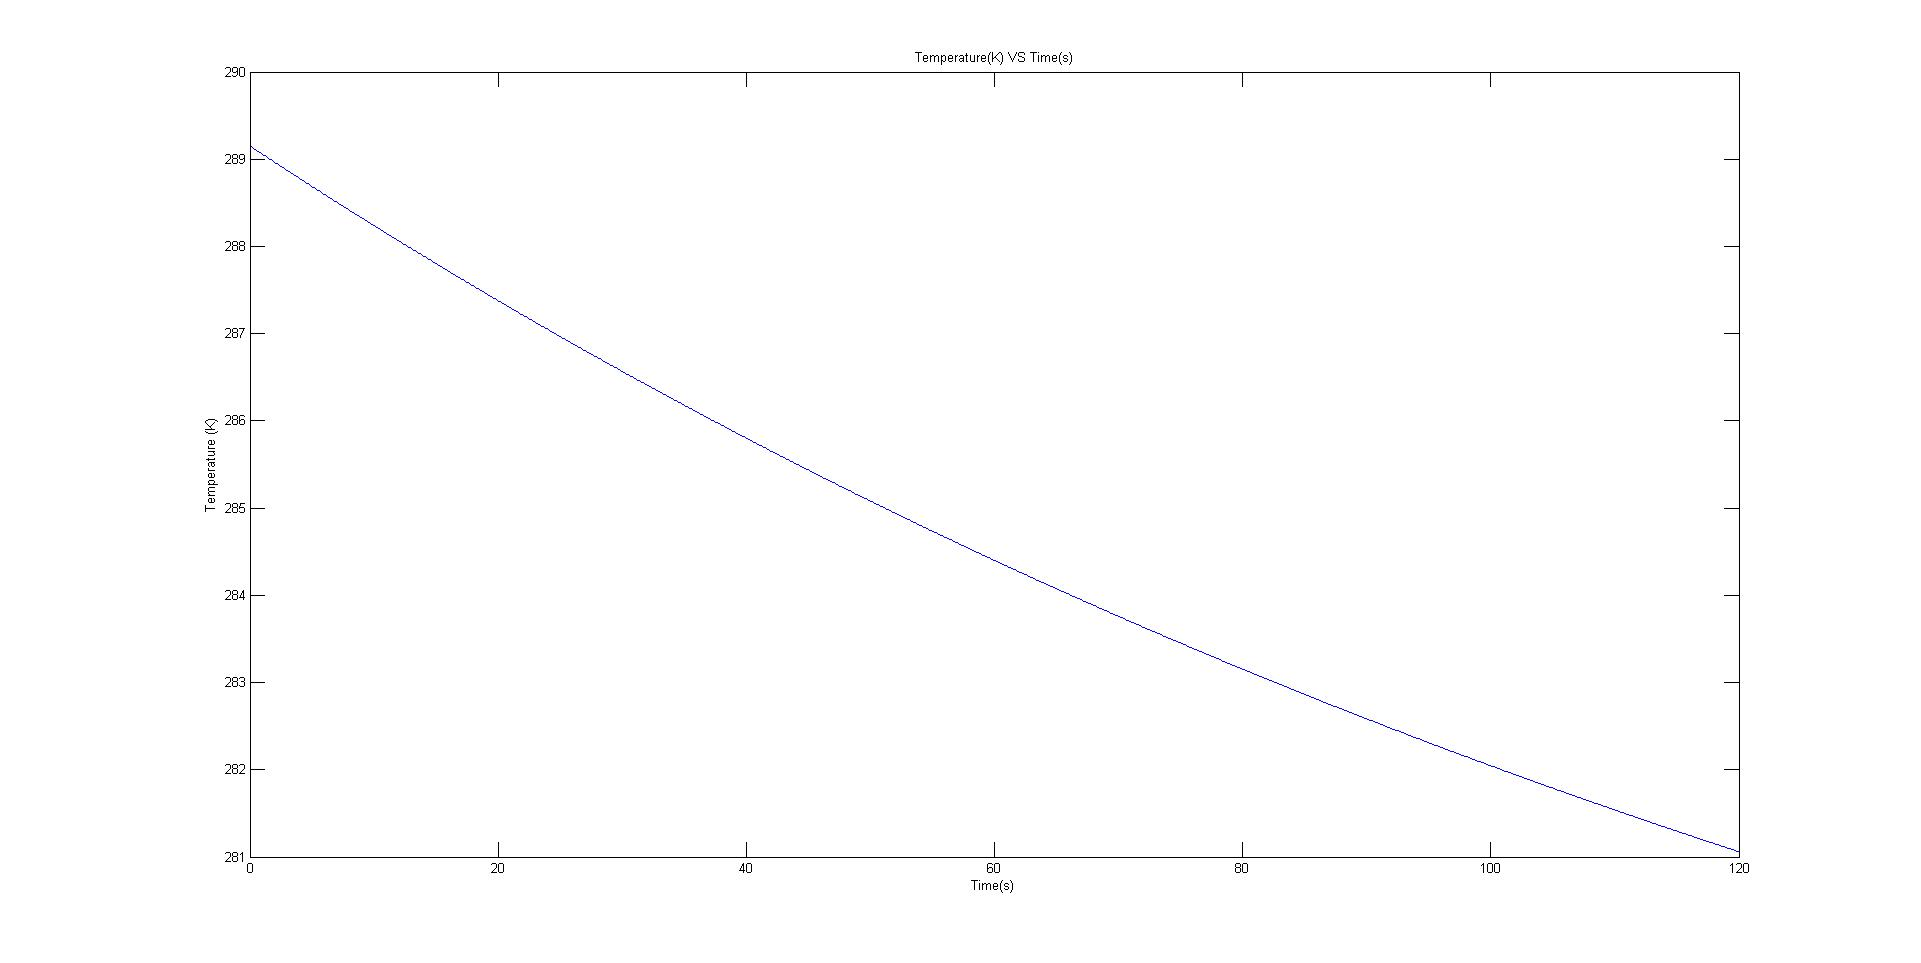
\includegraphics[width=\textwidth]{img/NSg.jpg}
		\caption{Graph of temperature versus time for the non-spinning can. The star marks the $60s$ point.}
		\label{NSg}
	\end{figure}
	
	
	
	\subsection{Spinning can}\label{sc}
	
	For this model, simplifying assumptions made in section~\ref{nsc} will be used, concerning Prandtl number ($Pr$), the density of water ($\rho$), the volume expansion coefficient for water ($\beta$), the specific heat of water ($C_p$) and thermal conductivity of water ($k$).
	
	In this case, the hot water cylinder shown in red on figure~\ref{cyl} is spinning at $\Omega=1000rpm=1.6667\times 10^1 \frac{rounds}{s}$. This can be considered as a flow along a plate, the plate being the interface between hot and cold water, at a certain speed $U$.
	
	The speed of cold water on the side of the water is not exactly equal to $U$. Indeed, water begins to spin around the can. The speed's distribution outside of the can is decreasing quickly, with a maximum on the can's surface. This maximum is given by $U_{max}= \Omega \pi d=3.4558\frac{m}{s}$. The speed quickly drops to zero since ice is slowing the water. The linear approximation made before will be used again and the flow will be considered as having a ``mean'' speed of $U=\frac{U_{max}}{2}=1.7279\frac{m}{s}$.
	
	Knowing this speed, the calculation of Reynolds number $Re=\frac{\rho U L}{\mu}$ can be made. The characteristic length $L$ for this problem is the circumference of the can, since the speed is tangent to the can, which gives $L=\pi d$. $\nu$ is the dynamic viscosity of water and can be found on table 9, Annex-1 of ``Heat and Mass Transfer: Fundamentals and Applications''~\cite{HaMT}. The same approach as before will be kept and the ``mean'' value of $\mu$ on the interval will be considered. This value is $\mu=1.2225\times 10^{-3}$. Reynolds is thus $\Re= \frac{999.4 \times 1.7279 \times 0.116}{1.2225\times 10^{-3}}= 1.6386 \times 10^5$.
	
	The next step is to use the formula for a flow on a flat plate (see annex~\ref{FORMU} page 4). The Reynolds number calculated before is $Re<3\times 10^5$, meaning that we are in laminar regime:
	\begin{equation}
		\begin{gathered}
		Nu_{out}= \frac{1}{2}0.332Pr^{\frac{1}{3}}\sqrt{Re}\\
		Nu_{out}=1.3857\times 10^2
		\end{gathered}
	\end{equation}
	
	$h$ can now be calculated :
	\begin{equation}
	h_{out}=\frac{Nu_{out}k}{L}=3.9029\times 10^2 \frac{W}{m^2K}
	\end{equation}
	
	Biot number is given by $Bi=\frac{h_{out}}{{\frac{4k}{d}+h_{in}}}$ where $h_{in}$ was calculated for natural convection in the non-spinning case~\ref{nsc}. Biot is thus $Bi=9.671\times 10^{-1}$, which is lower than the critical value of $1$. Using the lumped system equation~\ref{lumped} is therefore perfectly correct.

	With $h=h_{out}+h_{in}$ and for $t=60s$, the final temperature is $T=281.42K=8.27$\textcelsius.
	
	Graph~\ref{Sg} shows the relation between temperature and time for different rotation speeds, ranging from $\Omega=0rpm$ to $\Omega=1750rpm$, with steps of $250rpm$. It can clearly be observed that at higher speeds, the can is cooled down more quickly.
	
	\begin{figure}
		\centering
		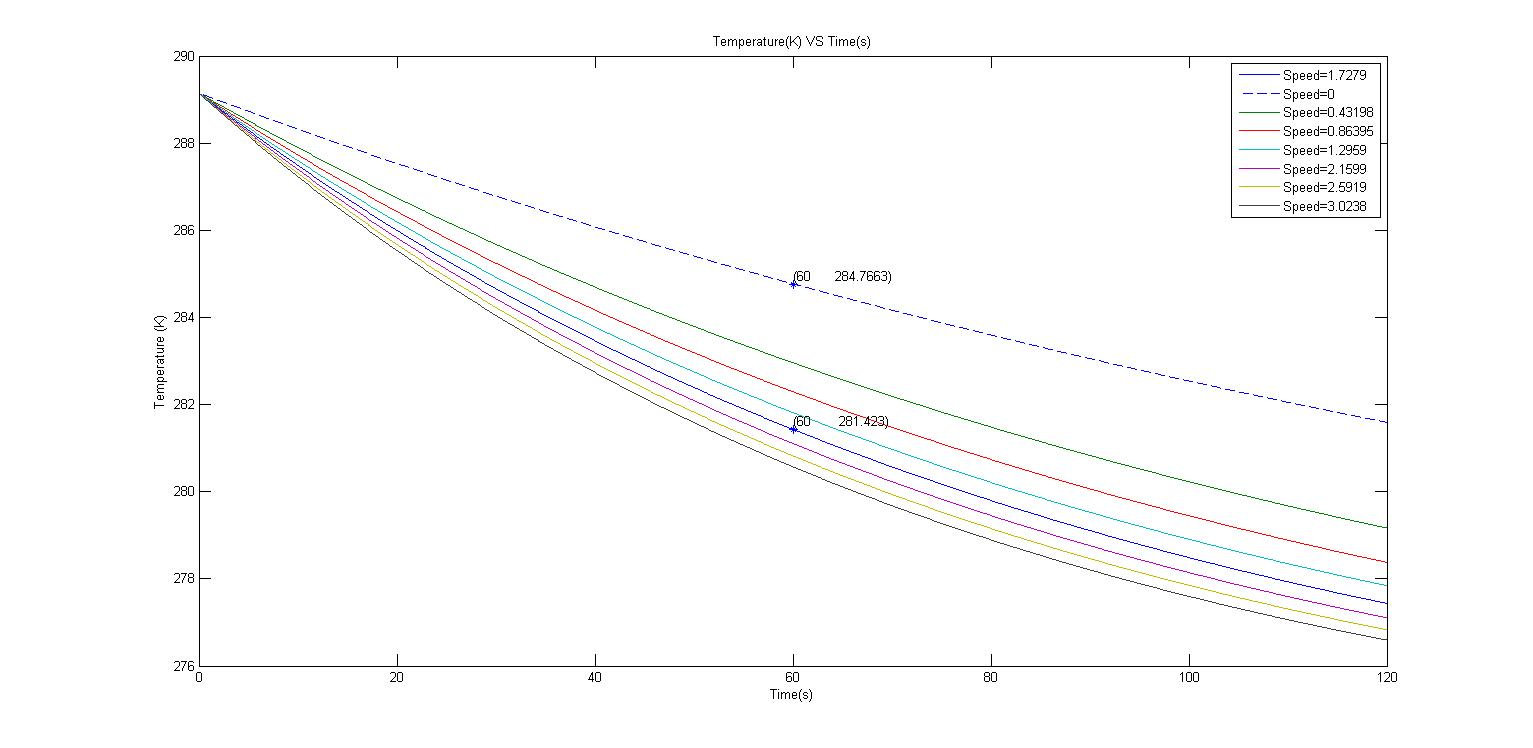
\includegraphics[width=\textwidth]{img/Sg.jpg}
		\caption{Graph of temperature versus time for the spinning can for speeds ranging from $\Omega=0rpm$ to $\Omega=1750rpm$, steps of $250rpm$}
		\label{Sg}
	\end{figure}
	
	\chapter[Reality and mathematical model]{Comparison between reality and the mathematical model}\label{rvmm}
	
	This section is about the difference between the mathematical model and the reality. A simple look at the measurement done underlines that the mathematical model does not perfectly correspond to the reality. The temperature observed in the non-spinning case are $11.9$ \textcelsius\ in reality and $11.61$ \textcelsius\ in the mathematical model. For the spinning case, they are respectively $11$ \textcelsius\  and $8.27$\textcelsius\.
	The main reason of this difference is that the mathematical model is based on simplified assumptions.
	
	The first one was to consider that the fluid inside	the can has the same properties as water. This approximation leads to errors on the value of some calculated parameters such as the kinematic viscosity	used to calculate the Grashof number. Moreover this number has a direct impact on the value of the convective coefficient $h$ because it is used to calculate the Nusselt number($N_{u}=\frac{hL}{k}$). 
	
	The second one is that the surface of the can is described as a perfect cylinder and that some part of the surface are not taken into account because their influence is negligible. This also leads to slight differences with the reality.
	
	However the result obtained before are close from the actual value, especially for the non-spinning case. The main difference	between the two cases is the velocity of the spinning can. Even if this velocity is measured with good precision, the mathematical model considers $V_{fluid}=V_{screwdriver}$ on the surface of the can and the viscosity of the fluid (reducing the speed) is not taken into account, leading to significant lack of precision in the calculation of the convective coefficient $h$. This inaccuracy can be explained by the sensitivity of the forced convection to the velocity of the fluid as shown in graph~\ref{Sg}.


	The precision of the measurement is an other point of argument. Indeed, the temperatures inside of the two cans were not measured at the same moment, allowing for the second can to warm up. Moreover the thermometer used had a non-negligible size compared to the can. It is then impossible to know the exact temperature on a point.
	Therefore the system has to be considered as homogeneous which is not exactly the case in actual practice.

	Finally, the experiment was only done once, we can thus not ensure we did not make any mistake during the manipulation. Concluding on the precision of our model compared to only one experiment would be presumptuous.

	\chapter{Conclusion}\label{ccl}
	
	As seen in the previous section there are differences between the theoretical model and the reality. These differences can be explained by the different approximations done in the model and by experimental errors. However, even if the mathematical model does not perfectly fit the reality, it puts in evidence the general behaviour of the system which is the point of this study.

	The general behaviour of the two different cases underlines the impact of forced convection, natural convection and conduction in heat transfers and on this basis some conclusion about heat transfer processes can be made.
	
	First, because of the flow properties of the fluid, the conductive heat transfer is negligible in comparison with convective heat transfers and can be omit.
	
	Then, it is necessary to distinguish natural and forced convection. As seen on the graph~\ref{Sg}, at high speed, forced convection becomes far more important than natural convection, which leads to the difference of final temperature in the two studied cases.
	
	Looking at this different phenomena with an engineer point of view, the possibilities offered by forced convection appear clearly relevant, not only for a can cooling systems but also in various other applications where it could accelerate heat transfer processes.
	
	\appendix

	\chapter{Water Thermo-Physical Properties}\label{WTPP}
	
	These chart can be are extracted from ``Perry’s	Chemical Engineers’ Handbook'', Chapter 2\cite{properties}.
	
	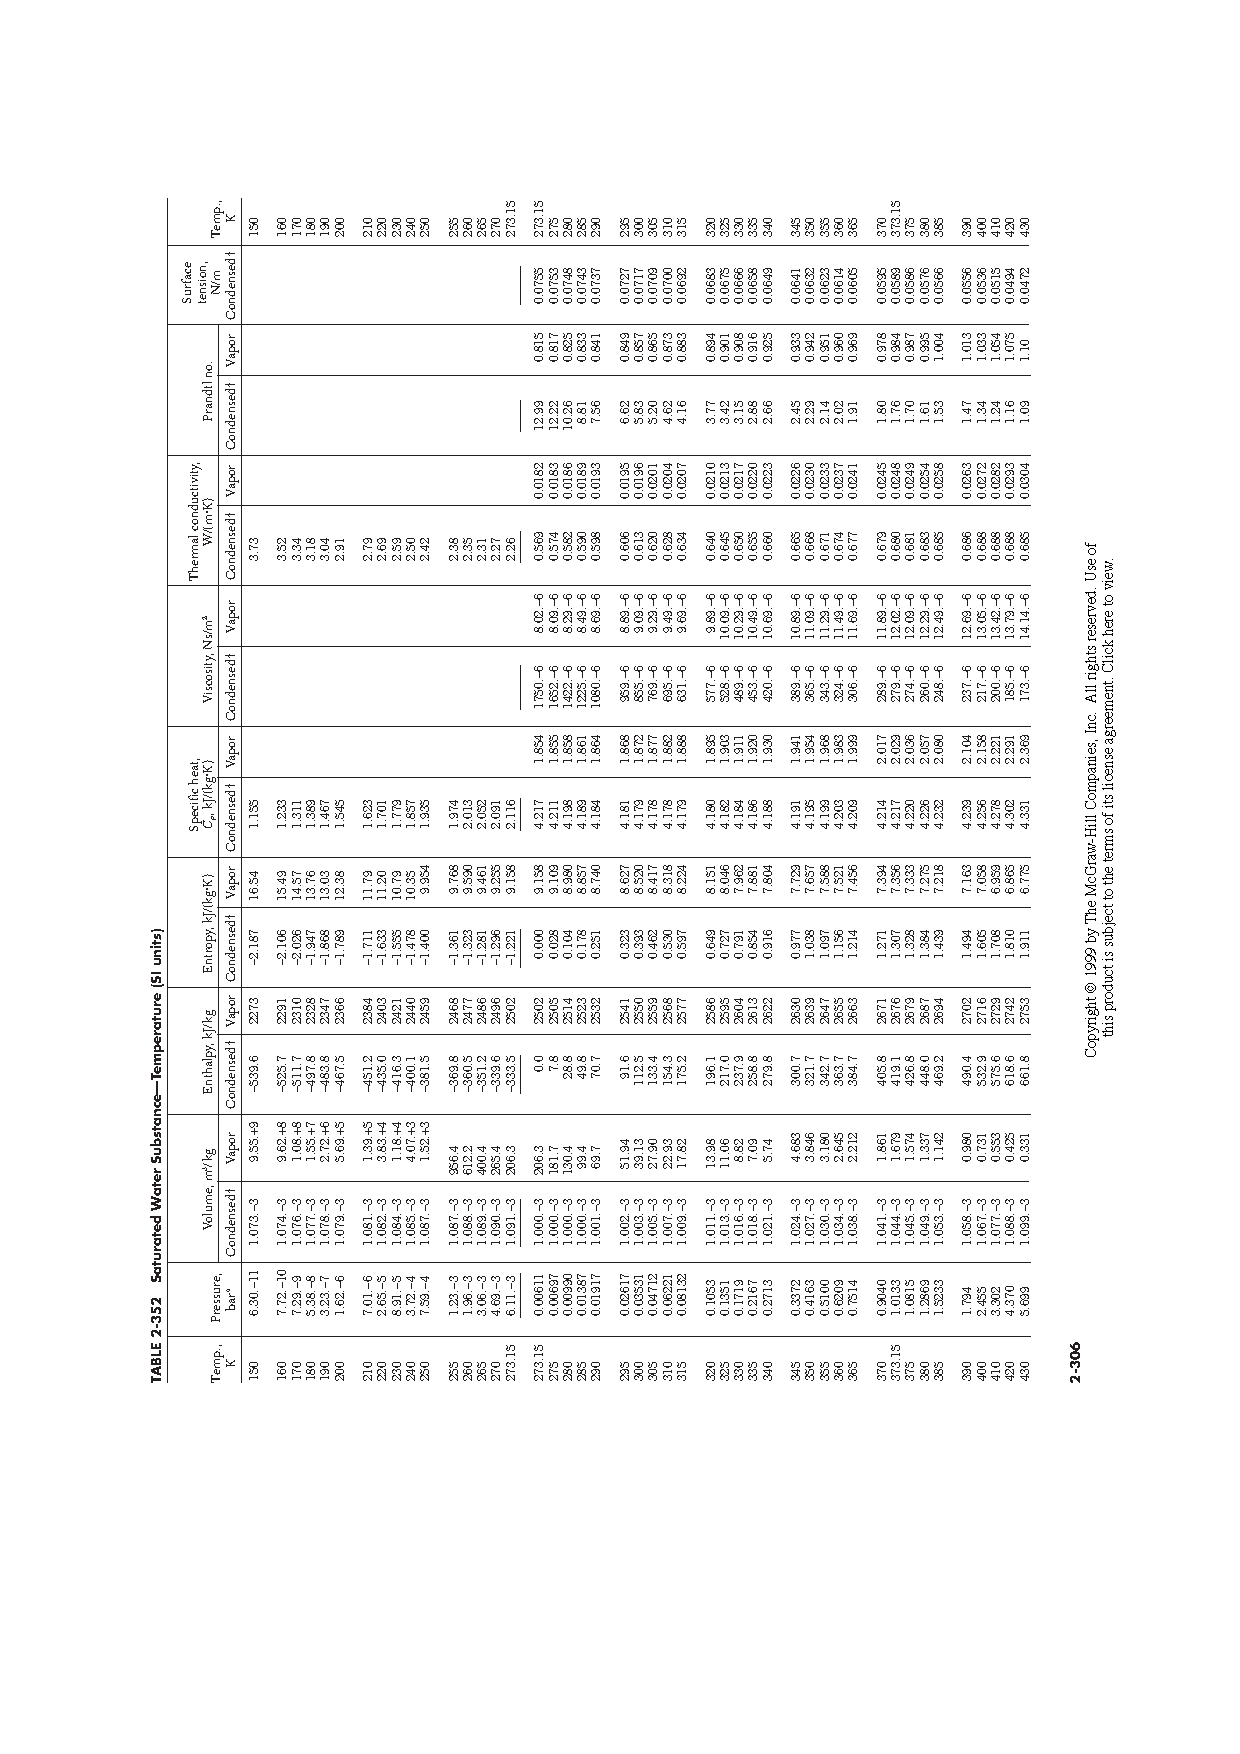
\includepdf[pages={-}]{WaterThermo-PhysicalProperties.pdf}
	
	\chapter{Formula Sheet}\label{FORMU}
	
	The following formula sheet was given and demonstrated at Pr. Parente's course ``MECA-H3001: Fluid mechanics and transfer processes''.
	
	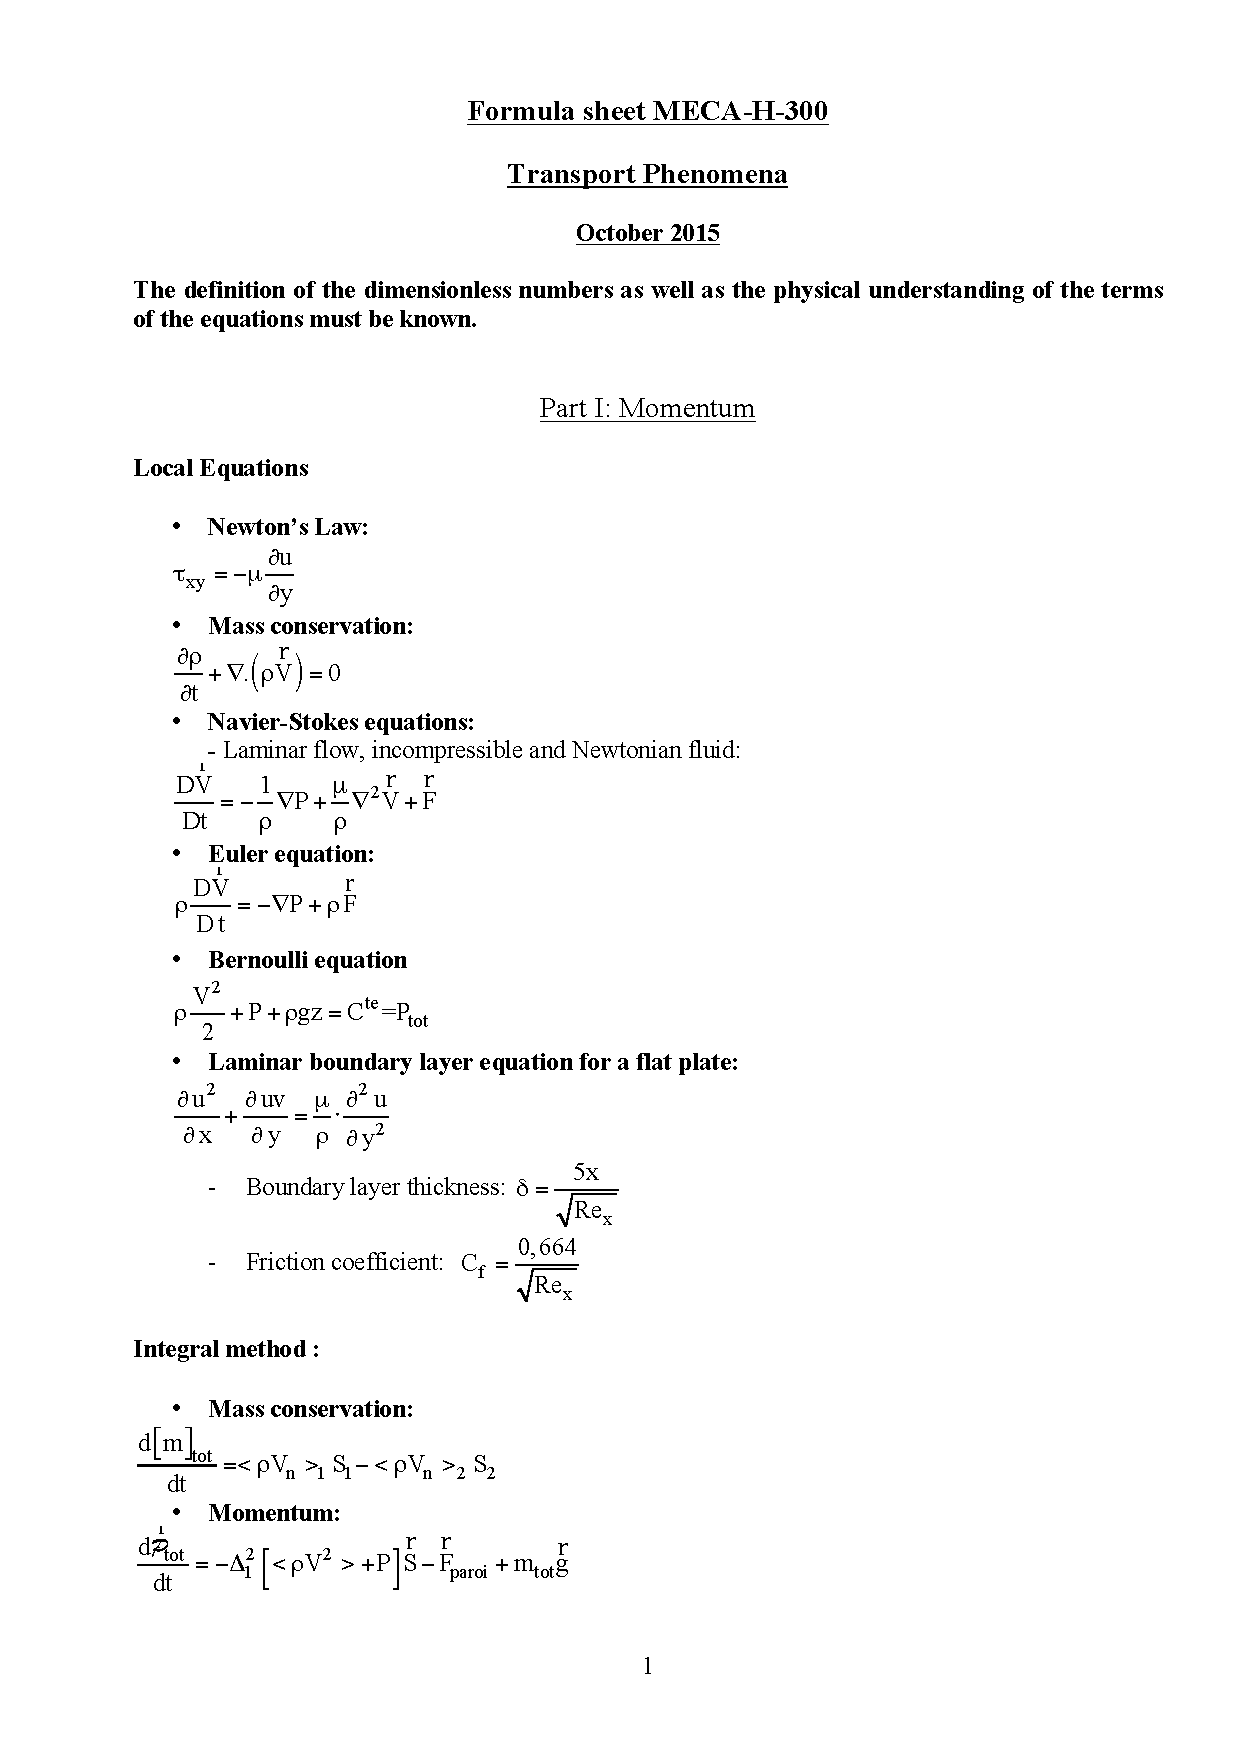
\includepdf[pages={-}]{FormulaSheet.pdf}
	
	\chapter{Codes}
	
	The following codes where used to calculate the models and obtain the different graphs. The reader should be advised this code is only usable for this work and should not be reused as it takes in account parameters and simplifying assumptions made for this particular experiment.
	
	\section{Non-spinning model}\label{codeNS}
	
	\begin{lstlisting}[style=Matlab-editor]
	t = linspace(0,120,1210);
	Pr=8.77;
	beta=1.056*10^(-4);
	rho=999.4;
	k=.584;
	Cp=4189.5;
	Ra=Pr*(beta*9.81*16*(.066)^(3))/(1.081*10^(-6))^2;
	Nu=0.22*(Pr*Ra/(0.2+Pr))^(0.28) *(0.116/0.033)^(-1/4);
	h=Nu*k/.033;
	T60=(16./(exp((4*h*60)/(rho*4184*.066))))
	Tf=273.15 +(16./(exp((4*h*t)/(rho*Cp*.066))));
	plot(t,Tf,60,T60+273.15,'*')
	strValues = num2str([60 T60+273.15]);
	text(60,T60+273.15,strcat('(',strValues,')'),'VerticalAlignment','bottom');
	title('Temperature(K) VS Time(s)')
	xlabel('Time(s)')
	ylabel('Temperature (K)')
	\end{lstlisting}
	
	\section{Non-spinning model}\label{codeS}
	
	\begin{lstlisting}[style=Matlab-editor]
	t = linspace(0,120,1210);
	Pr=8.77;
	beta=1.056*10^(-4);
	rho=999.4;
	k=.584;
	Cp=4189.5;
	mu=.0012225;
	U=1.7279;
	Ra=Pr*(beta*9.81*16*(.066)^(3))/(1.081*10^(-6))^2;
	Nuin=0.22*(Pr*Ra/(0.2+Pr))^(0.28) *(0.116/0.033)^(-1/4);
	hin=Nuin*k/.033;
	Re=rho*U*.116/mu;
	Nuout=.5*.332*Pr^(1/3)*sqrt(Re);
	hout=Nuout*k/.2073451151;
	h=hin+hout;
	T60=(16./(exp((4*h*60)/(rho*4184*.066))))
	Tf=273.15 +(16./(exp((4*h*t)/(rho*Cp*.066))));
	
	U0=0;
	Re0=rho*U0*.116/mu;
	Nuout0=.5*.332*Pr^(1/3)*sqrt(Re0);
	hout0=Nuout0*k/.2073451151;
	h0=hin+hout0;
	T600=(16./(exp((4*h0*60)/(rho*4184*.066))))
	Tf0=273.15 +(16./(exp((4*h0*t)/(rho*Cp*.066))));
	
	U2=.25*U;U3=.5*U;U4=.75*U;U5=1.25*U;U6=1.5*U;U7=1.75*U;
	Re2=rho*U2*.116/mu;Re3=rho*U3*.116/mu;Re4=rho*U4*.116/mu;Re5=rho*U5*.116/mu;Re6=rho*U6*.116/mu;Re7=rho*U7*.116/mu;
	Nuout2=.5*.332*Pr^(1/3)*sqrt(Re2);
	Nuout3=.5*.332*Pr^(1/3)*sqrt(Re3);
	Nuout4=.5*.332*Pr^(1/3)*sqrt(Re4);
	Nuout5=.5*.332*Pr^(1/3)*sqrt(Re5);
	Nuout6=.5*.332*Pr^(1/3)*sqrt(Re6);
	Nuout7=.5*.332*Pr^(1/3)*sqrt(Re7);
	hout2=Nuout2*k/.2073451151;
	hout3=Nuout3*k/.2073451151;
	hout4=Nuout4*k/.2073451151;
	hout5=Nuout5*k/.2073451151;
	hout6=Nuout6*k/.2073451151;
	hout7=Nuout7*k/.2073451151;
	h2=hin+hout2;h3=hin+hout3;h4=hin+hout4;h5=hin+hout5;h6=hin+hout6;h7=hin+hout7;
	Tf2=273.15 +(16./(exp((4*h2*t)/(rho*Cp*.066))));
	Tf3=273.15 +(16./(exp((4*h3*t)/(rho*Cp*.066))));
	Tf4=273.15 +(16./(exp((4*h4*t)/(rho*Cp*.066))));
	Tf5=273.15 +(16./(exp((4*h5*t)/(rho*Cp*.066))));
	Tf6=273.15 +(16./(exp((4*h6*t)/(rho*Cp*.066))));
	Tf7=273.15 +(16./(exp((4*h7*t)/(rho*Cp*.066))));
	
	
	plot(t,Tf,t,Tf0,'b--',t,Tf2,t,Tf3,t,Tf4,t,Tf5,t,Tf6,t,Tf7,60,T60+273.15,'b*',60,T600+273.15,'b*')
	strValues = num2str([60 T60+273.15]);
	text(60,T60+273.15,strcat('(',strValues,')'),'VerticalAlignment','bottom');
	strValues0 = num2str([60 T600+273.15]);
	text(60,T600+273.15,strcat('(',strValues0,')'),'VerticalAlignment','bottom');
	legend(strcat('Speed=',num2str(U)),strcat('Speed=',num2str(U0)),strcat('Speed=',num2str(U2)),strcat('Speed=',num2str(U3)),strcat('Speed=',num2str(U4)),strcat('Speed=',num2str(U5)),strcat('Speed=',num2str(U6)),strcat('Speed=',num2str(U7)));
	title('Temperature(K) VS Time(s)')
	xlabel('Time(s)')
	ylabel('Temperature (K)')
	\end{lstlisting}
	
	
	\bibliography{biblio}{}
	\bibliographystyle{plain}
	
\end{document}